\documentclass[a4paper,11pt]{report}

\usepackage{amsmath,amssymb}
\usepackage{fullpage}
\usepackage{graphicx}

\usepackage{bussproofs}
\usepackage{mathpartir}
\usepackage{prooftrees}
\usepackage{color}

\usepackage{tikz}
\usetikzlibrary{automata,positioning}

\newcommand*\circled[1]{\tikz[baseline=(char.base)]{
            \node[shape=circle,draw,inner sep=2pt] (char) {#1};}}

\makeatletter
\pgfmathdeclarefunction{alpha}{1}{%
  \pgfmathint@{#1}%
  \edef\pgfmathresult{\pgffor@alpha{\pgfmathresult}}%
}

\newcommand*{\until}{U}
\newcommand*{\disj}{\ ,\ }
\newcommand*{\A}{\square}  % Always
\newcommand*{\D}{\diamondsuit} % eventually

\newcommand*{\Pq}{(\top,\bot)}
\newcommand*{\pQ}{(\bot,\top)}
\newcommand*{\PQ}{(\top,\top)}
\newcommand*{\pq}{(\bot,\bot)}

% tikz
\usepackage{tikz}
\usetikzlibrary{snakes}

\author{Sylvain Julmy}
\date{\today}

\setlength{\parindent}{0pt}
\setlength{\parskip}{2.5pt}

\begin{document}

\begin{center}
\Large{
    Automata on Infinite Structure\\
    Fall 2018
  }
  
  \noindent\makebox[\linewidth]{\rule{\linewidth}{0.4pt}}
  Exercice Sheet 4

  \vspace*{1.4cm}

  Author : Sylvain Julmy
  \noindent\makebox[\linewidth]{\rule{\linewidth}{0.4pt}}

  \begin{flushleft}
    Professor : Ultes-Nitsche Ulrich
    
    Assistant : Stammet Christophe
  \end{flushleft}

  \noindent\makebox[\linewidth]{\rule{\textwidth}{1pt}}
\end{center}

\section*{Exercice 1}

\[R_1 = \]

\begin{center}
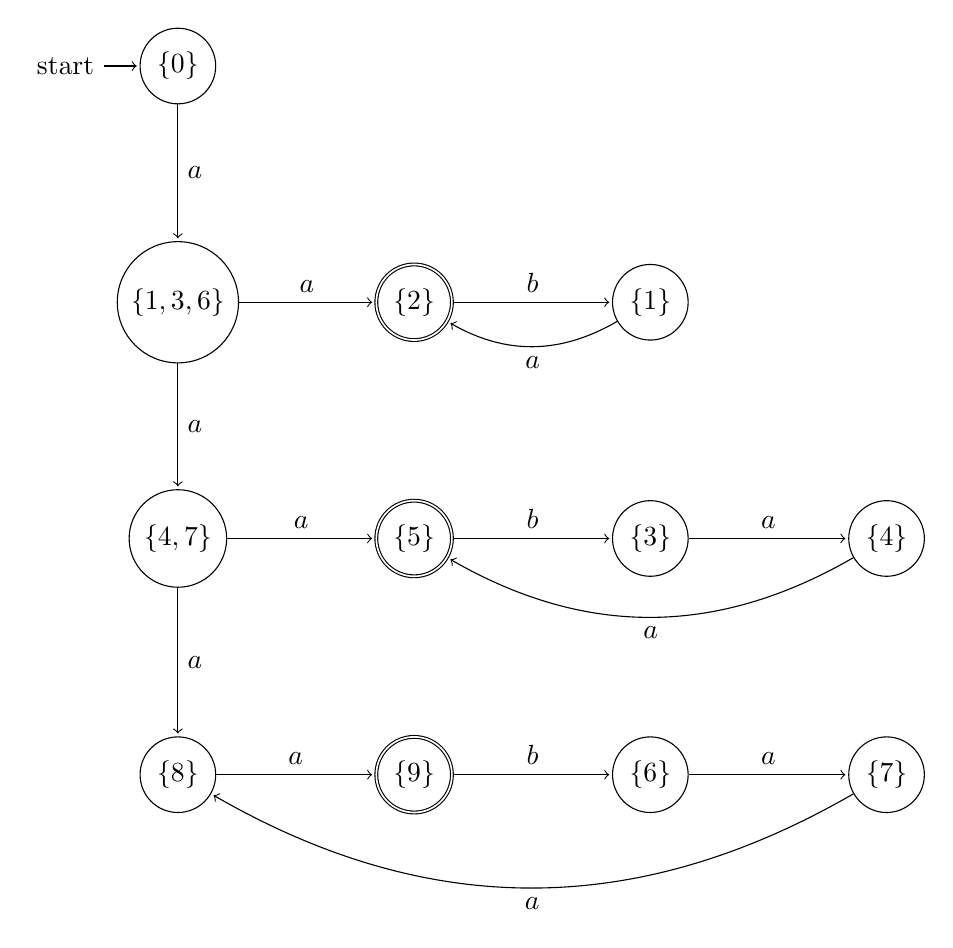
\begin{tikzpicture}[shorten >=1pt,node distance=3cm,on grid,auto]
  \node[state,initial] (q0) {$\{0\}$};
  \node[state] (q136) [below = of q0] {$\{1,3,6\}$};
  \node[state,accepting] (q2) [right = of q136] {$\{2\}$};
  \node[state] (q1) [right = of q2] {$\{1\}$};
  
  \node[state] (q47) [below = of q136] {$\{4,7\}$};
  \node[state,accepting] (q5) [right = of q47] {$\{5\}$};
  \node[state] (q3) [right = of q5] {$\{3\}$};
  \node[state] (q4) [right = of q3] {$\{4\}$};
  
  \node[state] (q8) [below = of q47] {$\{8\}$};
  \node[state,accepting] (q9) [right = of q8] {$\{9\}$};
  \node[state] (q6) [right = of q9] {$\{6\}$};
  \node[state] (q7) [right = of q6] {$\{7\}$};
  \path[->]
  (q0)
  edge [] node [] {$a$} (q136)
  (q136)
  edge [] node [] {$a$} (q2)
  edge [] node [] {$a$} (q47)
  (q47)
  edge [] node [] {$a$} (q5)
  edge [] node [] {$a$} (q8)
  (q1)
  edge [bend left] node [] {$a$} (q2)
  (q2)
  edge [] node [] {$b$} (q1)
  (q5)
  edge [] node [] {$b$} (q3)
  (q9)
  edge [] node [] {$b$} (q6)
  (q4)
  edge [bend left] node [] {$a$} (q5)
  (q7)
  edge [bend left] node [] {$a$} (q8)
  (q8)
  edge [] node [] {$a$} (q9)
  (q6)
  edge [] node [] {$a$} (q7)
  (q3)
  edge [] node [] {$a$} (q4)
  ;
\end{tikzpicture}
\end{center}

\[R_2 = \]

\begin{center}
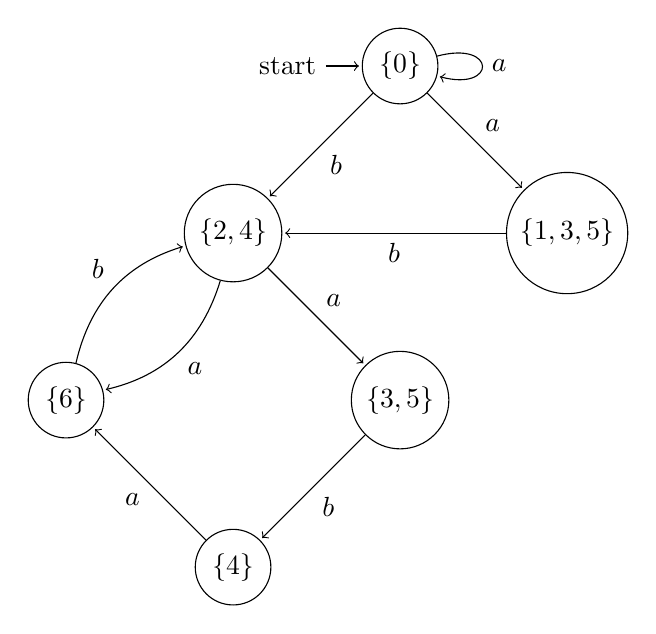
\begin{tikzpicture}[shorten >=1pt,node distance=3cm,on grid,auto]
  \node[state,initial] (q0) {$\{0\}$};
  \node[state] (q135) [below right = of q0] {$\{1,3,5\}$};
  \node[state] (q24) [below left = of q0] {$\{2,4\}$};
  \node[state] (q6) [below left = of q24] {$\{6\}$};
  \node[state] (q35) [below right = of q24] {$\{3,5\}$};
  \node[state] (q4) [below right = of q6] {$\{4\}$};
  \path[->]
  (q0)
  edge [loop right] node [] {$a$} ()
  edge [] node [] {$a$} (q135)
  edge [] node [] {$b$} (q24)
  (q135)
  edge [] node [] {$b$} (q24)
  (q24)
  edge [bend left] node [] {$a$} (q6)
  edge [] node [] {$a$} (q35)
  (q6)
  edge [bend left] node [] {$b$} (q24)
  (q35)
  edge [] node [] {$b$} (q4)
  (q4)
  edge [] node [] {$a$} (q6)
  ;
\end{tikzpicture}
\end{center}

\section*{Exercice 2}

$$ A = $$
\begin{center}
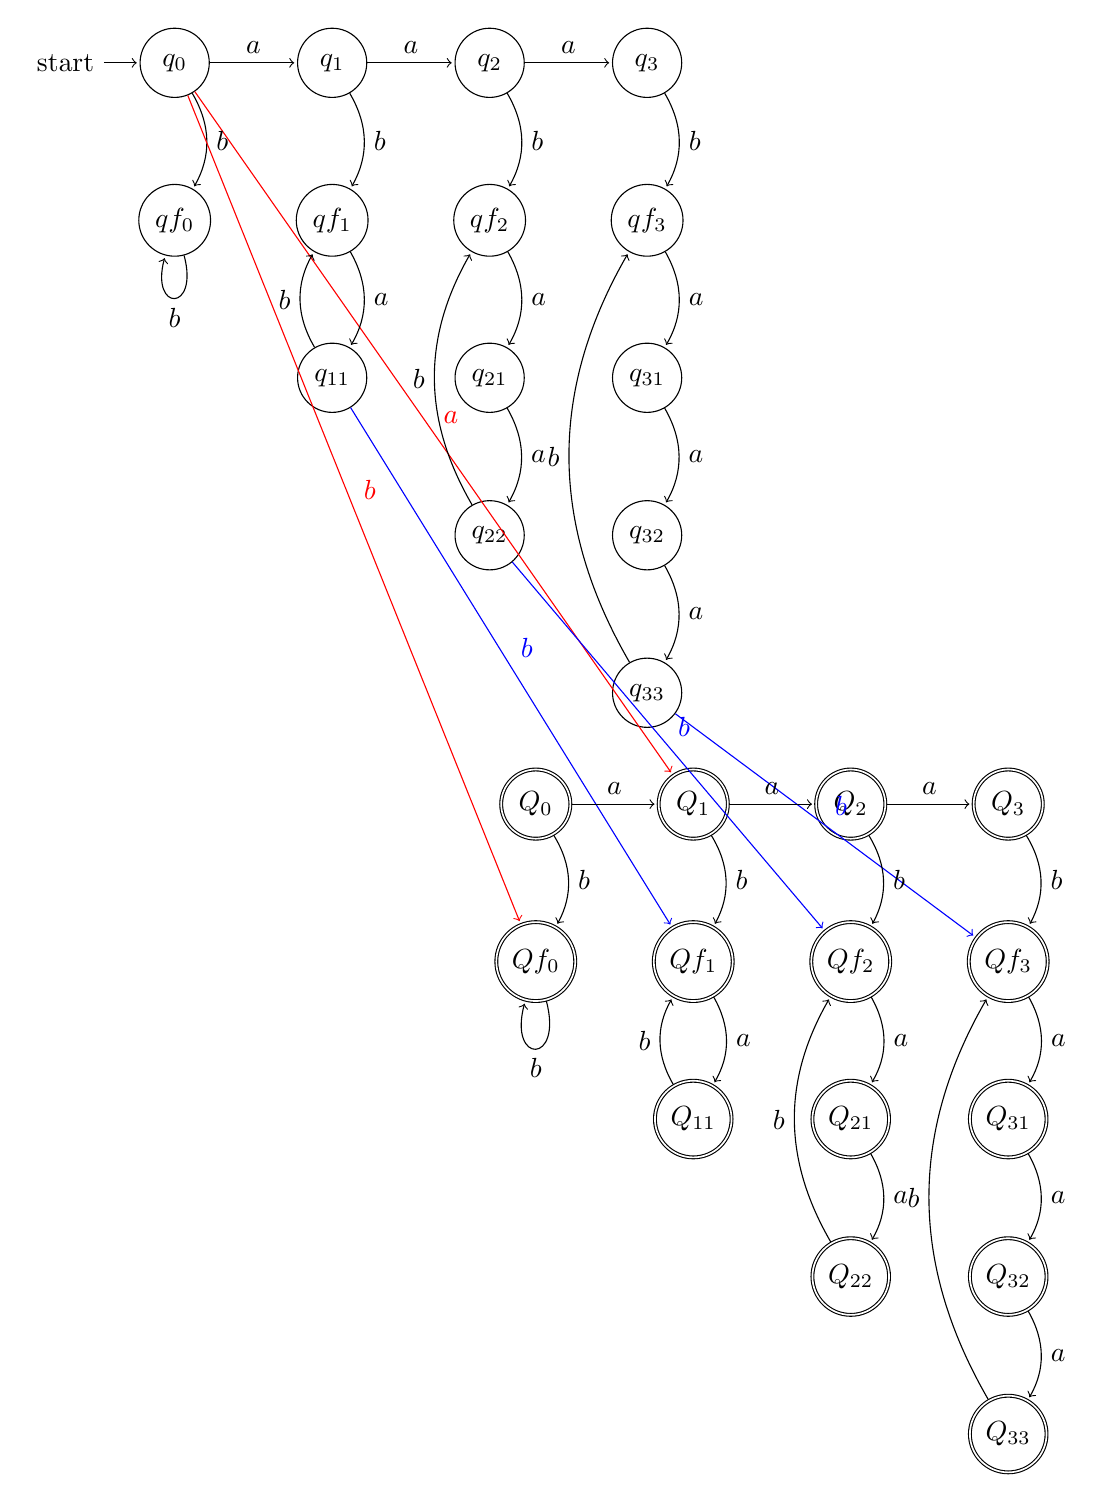
\begin{tikzpicture}[shorten >=1pt,node distance=2cm,on grid,auto]
  \node[state,initial] (q0) {$q_0$};
  \node[state] (q1) [right = of q0] {$q_1$};
  \node[state] (q2) [right = of q1] {$q_2$};
  \node[state] (q3) [right = of q2] {$q_3$};
  
  \node[state] (qf0) [below = of q0] {$qf_0$};
  \node[state] (qf1) [right = of qf0] {$qf_1$};
  \node[state] (qf2) [right = of qf1] {$qf_2$};
  \node[state] (qf3) [right = of qf2] {$qf_3$};
  
  \node[state] (q11) [below = of qf1] {$q_{11}$};
  \node[state] (q21) [below = of qf2] {$q_{21}$};
  \node[state] (q31) [below = of qf3] {$q_{31}$};
  
  \node[state] (q22) [below = of q21] {$q_{22}$};
  \node[state] (q32) [below = of q31] {$q_{32}$};
  
  \node[state] (q33) [below = of q32] {$q_{33}$};

  \node[state,accepting] (Q0) [below left = of q33]{$Q_0$};
  \node[state,accepting] (Q1) [right = of Q0] {$Q_1$};
  \node[state,accepting] (Q2) [right = of Q1] {$Q_2$};
  \node[state,accepting] (Q3) [right = of Q2] {$Q_3$};
  
  \node[state,accepting] (Qf0) [below = of Q0] {$Qf_0$};
  \node[state,accepting] (Qf1) [right = of Qf0] {$Qf_1$};
  \node[state,accepting] (Qf2) [right = of Qf1] {$Qf_2$};
  \node[state,accepting] (Qf3) [right = of Qf2] {$Qf_3$};
  
  \node[state,accepting] (Q11) [below = of Qf1] {$Q_{11}$};
  \node[state,accepting] (Q21) [below = of Qf2] {$Q_{21}$};
  \node[state,accepting] (Q31) [below = of Qf3] {$Q_{31}$};
  
  \node[state,accepting] (Q22) [below = of Q21] {$Q_{22}$};
  \node[state,accepting] (Q32) [below = of Q31] {$Q_{32}$};
  
  \node[state,accepting] (Q33) [below = of Q32] {$Q_{33}$};

  
  \path[->]
  (q0)
  edge [] node [] {$a$} (q1)
  edge [red] node [] {$a$} (Q1)
  edge [bend left] node [] {$b$} (qf0)
  edge [red] node [] {$b$} (Qf0)
  (qf0)
  edge [loop below] node [] {$b$} ()
  (qf1)
  edge [bend left] node [] {$a$} (q11)
  (qf2)
  edge [bend left] node [] {$a$} (q21)
  (qf3)
  edge [bend left] node [] {$a$} (q31)
  (q21)
  edge [bend left] node [] {$a$} (q22)
  (q31)
  edge [bend left] node [] {$a$} (q32)
  (q32)
  edge [bend left] node [] {$a$} (q33)
  (q1)
  edge [] node [] {$a$} (q2)
  edge [bend left] node [] {$b$} (qf1)
  (q2)
  edge [] node [] {$a$} (q3)
  edge [bend left] node [] {$b$} (qf2)
  (q3)
  edge [bend left] node [] {$b$} (qf3)
  (q11)
  edge [bend left] node [] {$b$} (qf1)
  edge [blue] node [] {$b$} (Qf1)
  (q22)
  edge [bend left] node [] {$b$} (qf2)
  edge [blue] node [] {$b$} (Qf2)
  (q33)
  edge [bend left] node [] {$b$} (qf3)
  edge [blue] node [] {$b$} (Qf3)
  ;


  
  \path[->]
  (Q0)
  edge [] node [] {$a$} (Q1)
  edge [bend left] node [] {$b$} (Qf0)
  (Qf0)
  edge [loop below] node [] {$b$} ()
  (Qf1)
  edge [bend left] node [] {$a$} (Q11)
  (Qf2)
  edge [bend left] node [] {$a$} (Q21)
  (Qf3)
  edge [bend left] node [] {$a$} (Q31)
  (Q21)
  edge [bend left] node [] {$a$} (Q22)
  (Q31)
  edge [bend left] node [] {$a$} (Q32)
  (Q32)
  edge [bend left] node [] {$a$} (Q33)
  (Q1)
  edge [] node [] {$a$} (Q2)
  edge [bend left] node [] {$b$} (Qf1)
  (Q2)
  edge [] node [] {$a$} (Q3)
  edge [bend left] node [] {$b$} (Qf2)
  (Q3)
  edge [bend left] node [] {$b$} (Qf3)
  (Q11)
  edge [bend left] node [] {$b$} (Qf1)
  (Q22)
  edge [bend left] node [] {$b$} (Qf2)
  (Q33)
  edge [bend left] node [] {$b$} (Qf3)
  ;
\end{tikzpicture}
\end{center}

Note : not all transitions from the original DBA and the new one are indicated
because the pictures would be absolutely a nightmare to read. Some transitions
from the original one to the new one are indicated in color (It's the same for exercice 3).

Thus, I am realy not sure about my construction, I follow the instructions but
it's not really clear for me... (It's the same for exercice 3).

\section*{Exercice 3}

\begin{center}
  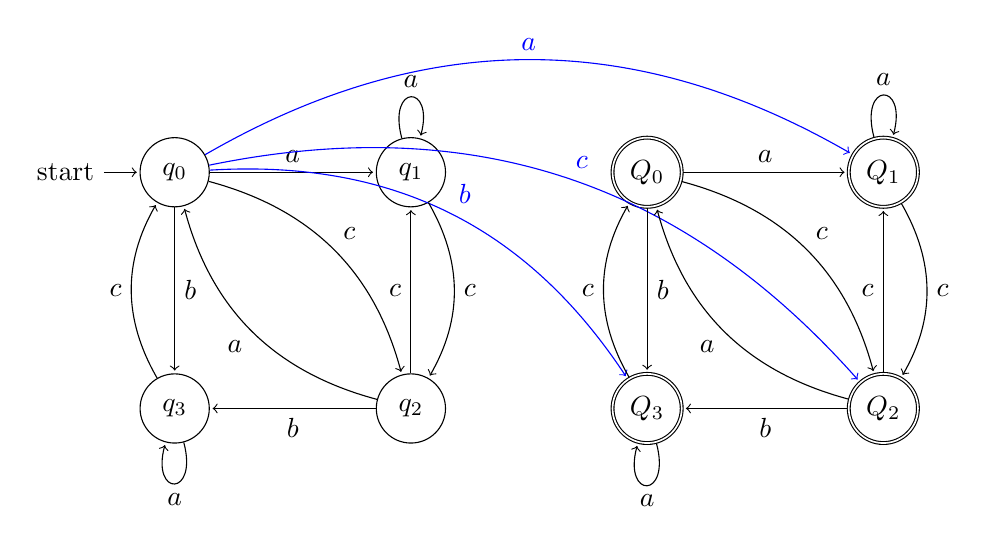
\begin{tikzpicture}[shorten >=1pt,node distance=3cm,on grid,auto]
    \node[state,initial] (q0) {$q_0$};
    \node[state] (q1) [right = of q0] {$q_1$};
    \node[state] (q2) [below = of q1] {$q_2$};
    \node[state] (q3) [left = of q2] {$q_3$};

    \node[state,accepting] (Q0) [right = of q1] {$Q_0$};
    \node[state,accepting] (Q1) [right = of Q0] {$Q_1$};
    \node[state,accepting] (Q2) [below = of Q1] {$Q_2$};
    \node[state,accepting] (Q3) [left = of Q2] {$Q_3$};
    
    \path[->]
    (q0)
    edge [] node [] {$a$} (q1)
    edge [blue, bend left] node [] {$a$} (Q1)
    edge [] node [] {$b$} (q3)
    edge [blue, bend left] node [] {$b$} (Q3)
    edge [bend left] node [] {$c$} (q2)
  edge [blue, bend left] node [] {$c$} (Q2)
  (q1)
  edge [loop above] node [] {$a$} ()
  edge [bend left] node [] {$c$} (q2)
  (q2)
    edge [] node [] {$c$} (q1)
    edge [bend left] node [] {$a$} (q0)
    edge [] node [] {$b$} (q3)
    (q3)
    edge [loop below] node [] {$a$} ()
    edge [bend left] node [] {$c$} (q0)
    (Q0)
    edge [] node [] {$a$} (Q1)
    edge [] node [] {$b$} (Q3)
    edge [bend left] node [] {$c$} (Q2)
    (Q1)
    edge [loop above] node [] {$a$} ()
    edge [bend left] node [] {$c$} (Q2)
    (Q2)
    edge [] node [] {$c$} (Q1)
    edge [bend left] node [] {$a$} (Q0)
    edge [] node [] {$b$} (Q3)
    (Q3)
    edge [loop below] node [] {$a$} ()
    edge [bend left] node [] {$c$} (Q0)

    ;
  \end{tikzpicture}
\end{center}


\end{document}